\chapter{Symétrie d’échange, spin et les deux signes moins}

\section{Remplissage des couches et question des statistiques de spin--}

Le rappel du modèle en couches commence par deux propriétés des électrons. Un électron a un spin égal à un demi, dont les deux projections de spin sans dimension sont
\begin{equation}
m_s=+\frac12,
\qquad
m_s=-\frac12,
\end{equation}
et les électrons obéissent au principe d’exclusion de Pauli. Ces faits sont liés, mais ils ne constituent pas une seule et même affirmation.

L’expression ``le même état'' demande quelques précisions. Deux électrons ne peuvent pas occuper le même état complet à une particule. Ils peuvent néanmoins partager la même orbitale spatiale si leurs états de spin diffèrent. Dans l’approximation des électrons indépendants appliquée à l’hélium, les deux électrons occupent l’orbitale spatiale de plus basse énergie, l’un avec le spin vers le haut et l’autre avec le spin vers le bas. Plus précisément, les possibilités ``le premier a le spin vers le haut et le second vers le bas'' et ``le premier a le spin vers le bas et le second vers le haut'' appartiennent à un état de spin intriqué des deux électrons.

Il ne s’agit que de l’ancien modèle en couches dans son approximation. Celui-ci néglige l’interaction entre les électrons et sert ici à un simple dénombrement. Pour le lithium, les deux premiers électrons remplissent l’orbitale spatiale de plus basse énergie avec des spins opposés. Le troisième ne peut entrer dans aucun de ces deux états complets et doit occuper une orbitale de plus haute énergie.

L’étape suivante est le diagramme familier du moment cinétique orbital. Les secteurs pour lesquels
\begin{equation}
\ell=0,\qquad \ell=1,\qquad \ell=2
\end{equation}
sont appelés états \(S\), \(P\) et \(D\). Une valeur fixée de \(\ell\) comporte
\begin{equation}
2\ell+1
\end{equation}
états orbitaux, donc
\begin{equation}
\ell=0\Rightarrow 1,
\qquad
\ell=1\Rightarrow 3,
\qquad
\ell=2\Rightarrow 5.
\end{equation}
Le problème coulombien présente des dégénérescences supplémentaires : des niveaux radiaux de secteurs \(\ell\) différents peuvent avoir la même énergie. Pour le raisonnement sur le remplissage des couches, la couche suivante contient une orbitale \(S\) et trois orbitales \(P\). Elle comporte donc
\begin{equation}
1+3=4
\end{equation}
états spatiaux. Le spin double ce nombre :
\begin{equation}
2(1+3)=8.
\end{equation}

Ces huit états complets à un électron se remplissent selon la progression simple qui va du lithium au néon. Au-delà de la couche fermée, le sodium possède de nouveau un électron externe, ce qui explique pourquoi cette représentation grossière le fait ressembler au lithium. La chimie n’est pas le but recherché. L’essentiel est que le spin demi-entier et l’exclusion apparaissent ensemble.

Les photons offrent un contraste. Ils ont un spin entier et ne sont soumis à aucune règle d’exclusion. Une onde électromagnétique classique correspond à de nombreux photons occupant le même mode. Les bosons peuvent s’accumuler dans un même état, tandis que des fermions identiques ne peuvent occuper plus d’une fois un même état complet. La question est de savoir si ces deux associations auraient pu être inversées : un spin demi-entier sans exclusion, ou un spin entier avec exclusion. En trois dimensions spatiales, la relation spin--statistiques répond par la négative. L’affirmation familière doit être nuancée dans une et deux dimensions spatiales, et aucune preuve du résultat de théorie des champs n’est présentée ici.

\begin{classroomqa}
\lecturetimestamp{00:11:48}
\audiencequestion{Existe-t-il un nombre maximal de quanta bosoniques pouvant occuper un état ?}
\lecturerresponse{Non. Les bosons n’ont aucune limite d’occupation et tendent à s’accumuler dans un même état.}
\end{classroomqa}

\section{Fonctions d’onde à plusieurs particules}

Nous allons aborder ce lien à travers deux signes moins, l’un provenant de l’échange et l’autre de la rotation. Commençons par l’échange et mettons provisoirement le spin de côté.

Soit \(x_i\) la position de la particule \(i\). L’indice désigne une étiquette de particule, et non une composante cartésienne ; les trois coordonnées spatiales sont condensées dans le symbole unique \(x_i\). Une base de position pour \(n\) particules est
\begin{equation}
\lvert x_1,x_2,\ldots,x_n\rangle.
\end{equation}
Pour un état abstrait \(\lvert\Psi\rangle\), la fonction d’onde en coordonnées est
\begin{equation}
\psi(x_1,x_2,\ldots,x_n)
=
\langle x_1,x_2,\ldots,x_n\mid\Psi\rangle.
\end{equation}
Son module au carré,
\begin{equation}
\bigl\lvert\psi(x_1,x_2,\ldots,x_n)\bigr\rvert^2,
\end{equation}
est la densité de probabilité conjointe de trouver la particule \(1\) en \(x_1\), la particule \(2\) en \(x_2\), et ainsi de suite.

Supposons maintenant que les particules soient identiques. Imaginons d’abord qu’on peigne un électron en bleu et un autre en rouge. On pourrait alors distinguer ``le bleu en \(x_1\) et le rouge en \(x_2\)'' de ``le bleu en \(x_2\) et le rouge en \(x_1\).'' En réalité, les électrons ne portent ni ces couleurs ni d’étiquettes individuelles de ce genre. Intervertir les étiquettes utilisées pour le calcul ne peut pas créer une nouvelle configuration physique.

Une phase globale ne modifie ni les probabilités ni les valeurs moyennes. Pour un état appartenant à un secteur d’échange défini, la fonction d’onde en coordonnées peut donc vérifier
\begin{equation}
\psi(x_2,x_1)=\eta\,\psi(x_1,x_2),
\qquad
\lvert\eta\rvert=1.
\end{equation}
Appliquer deux fois le même échange rétablit les arguments initiaux et donne
\begin{equation}
\eta^2=1,
\end{equation}
Les deux valeurs propres d’échange possibles sont donc
\begin{equation}
\eta=+1
\qquad\hbox{or}\qquad
\eta=-1.
\end{equation}

\editorialnote{L’algèbre du double échange détermine les valeurs propres possibles seulement après avoir supposé que l’état a un comportement défini sous l’échange. La restriction supplémentaire selon laquelle les états permis d’une espèce donnée appartiennent à un seul secteur d’échange est une règle physique ; elle ne découle pas de \(\eta^2=1\) à elle seule. La même réserve s’applique à l’argument d’exclusion ci-dessous : l’antisymétrie implique l’exclusion une fois le secteur fermionique choisi, mais l’algèbre de l’échange ne choisit pas ce secteur.}

Pour les bosons, les fonctions d’onde permises sont symétriques,
\begin{equation}
\psi_B(x_1,x_2)=\psi_B(x_2,x_1),
\end{equation}
tandis que pour les fermions, elles sont antisymétriques,
\begin{equation}
\psi_F(x_1,x_2)=-\psi_F(x_2,x_1).
\end{equation}
Le signe moins est invisible lorsqu’il multiplie l’état entier, mais il compte lorsque les amplitudes s’additionnent. C’est ainsi que la symétrie d’échange produit des conséquences observables.

\section{Produits, sommes et exclusion}

Considérons d’abord deux particules affectées à la même orbitale à une particule \(\psi_0\). Leur produit est
\begin{equation}
\psi_0(x_1)\psi_0(x_2).
\end{equation}
L’échange des coordonnées des particules donne
\begin{equation}
\psi_0(x_2)\psi_0(x_1)
=
\psi_0(x_1)\psi_0(x_2).
\end{equation}
Les valeurs d’une fonction d’onde sont des nombres, et non des opérateurs ; les facteurs commutent donc. Le produit correspondant au même état est symétrique. Il s’agit d’une forme permise pour des bosons, mais elle ne peut pas décrire deux fermions identiques.

Affectons ensuite les particules à des orbitales à une particule différentes :
\begin{equation}
\psi_0(x_1)\psi_1(x_2).
\end{equation}
L’échange donne
\begin{equation}
\psi_0(x_2)\psi_1(x_1).
\end{equation}
Si les fonctions sont distinctes, le produit échangé n’est en général ni l’expression initiale ni son opposé. Le produit brut ne possède donc aucune des deux symétries d’échange requises. Cela n’interdit pas à une particule d’occuper \(\psi_0\) pendant qu’une autre occupe \(\psi_1\). Cela signifie que l’état à deux particules doit combiner les deux affectations.

La combinaison symétrique est
\begin{equation}
\psi_B^{(01)}(x_1,x_2)
\propto
\psi_0(x_1)\psi_1(x_2)
+
\psi_0(x_2)\psi_1(x_1),
\end{equation}
et la combinaison antisymétrique est
\begin{equation}
\psi_F^{(01)}(x_1,x_2)
\propto
\psi_0(x_1)\psi_1(x_2)
-
\psi_0(x_2)\psi_1(x_1).
\end{equation}
Les signes de proportionnalité suffisent, car l’argument sur l’échange ne nécessite aucune normalisation. Ces deux états contiennent une particule dans chaque orbitale ; ils diffèrent uniquement par la façon dont sont combinées les deux affectations indiscernables.

Faisons maintenant coïncider les orbitales. La combinaison bosonique devient
\begin{align}
\psi_B^{(00)}(x_1,x_2)
&\propto
\psi_0(x_1)\psi_0(x_2)
+
\psi_0(x_2)\psi_0(x_1)\\
&=
2\psi_0(x_1)\psi_0(x_2),
\end{align}
qui n’est pas nulle. La combinaison fermionique donne
\begin{align}
\psi_F^{(00)}(x_1,x_2)
&\propto
\psi_0(x_1)\psi_0(x_2)
-
\psi_0(x_2)\psi_0(x_1)\\
&=0.
\end{align}
Avec la règle d’échange antisymétrique, l’exclusion s’ensuit : aucun état antisymétrique non nul ne peut avoir les deux fermions dans le même état à une particule.

Pour un état à plusieurs particules, la règle s’applique à toute transposition de deux arguments. Une transposition laisse une fonction d’onde bosonique inchangée et change le signe d’une fonction fermionique. Répéter la même transposition ne produit aucun effet dans les deux cas. Ce qui est surprenant, c’est qu’un échange unique, bien qu’il ne change aucune étiquette observable des particules, change le signe d’un état fermionique.

\section{Le spin dans l’étiquette complète d’une particule}

On peut maintenant réintroduire le spin avec une légère modification. Une amplitude à une particule dépend à la fois de la position et d’une étiquette de spin discrète,
\begin{equation}
\psi(x,\sigma),
\end{equation}
où \(\sigma=+1\) ou \(-1\) indique le résultat choisi de \(\sigma_z\). Le module au carré est la densité de probabilité conjointe pour la position et l’étiquette de spin indiquées.

Pour plusieurs particules, la fonction d’onde est
\begin{equation}
\psi(x_1,\sigma_1;\,x_2,\sigma_2;\,\ldots).
\end{equation}
L’échange permute tout ce qui appartient aux deux particules, et pas seulement leurs positions :
\begin{align}
\psi_B(x_1,\sigma_1;\,x_2,\sigma_2)
&=
+\psi_B(x_2,\sigma_2;\,x_1,\sigma_1),\\
\psi_F(x_1,\sigma_1;\,x_2,\sigma_2)
&=
-\psi_F(x_2,\sigma_2;\,x_1,\sigma_1).
\end{align}
C’est la formulation précise de l’affirmation initiale du modèle en couches. Deux électrons ne peuvent partager une même orbitale spatiale que si leurs états complets, spin compris, sont différents.

\begin{classroomqa}
\lecturetimestamp{00:34:33}
\audiencequestion{La symétrie d’échange est-elle un exemple du groupe des permutations ?}
\lecturerresponse{Oui. L’échange de particules est une permutation, et la loi de transformation avec un signe plus ou moins fournit une représentation du groupe des permutations.}
\end{classroomqa}

\begin{classroomqa}
\lecturetimestamp{00:35:12}
\audiencequestion{Pourquoi la construction à deux particules fait-elle intervenir un produit plutôt qu’une somme des fonctions d’onde à une particule ?}
\lecturerresponse{Une somme décrit une particule dans une superposition. Un produit appartient à l’espace produit tensoriel à deux particules et décrit une particule affectée à chacun des deux états à une particule.}
\end{classroomqa}

L’échange de toutes les étiquettes est illustré au tableau ci-dessous.\footnote{L’ordre des étiquettes de position--spin est reconstitué à partir de la partie lisible de l’image du tableau et de l’explication qui l’entoure, entre 00:33:43 et 00:34:25.}
\begin{figure}[htbp]
\centering
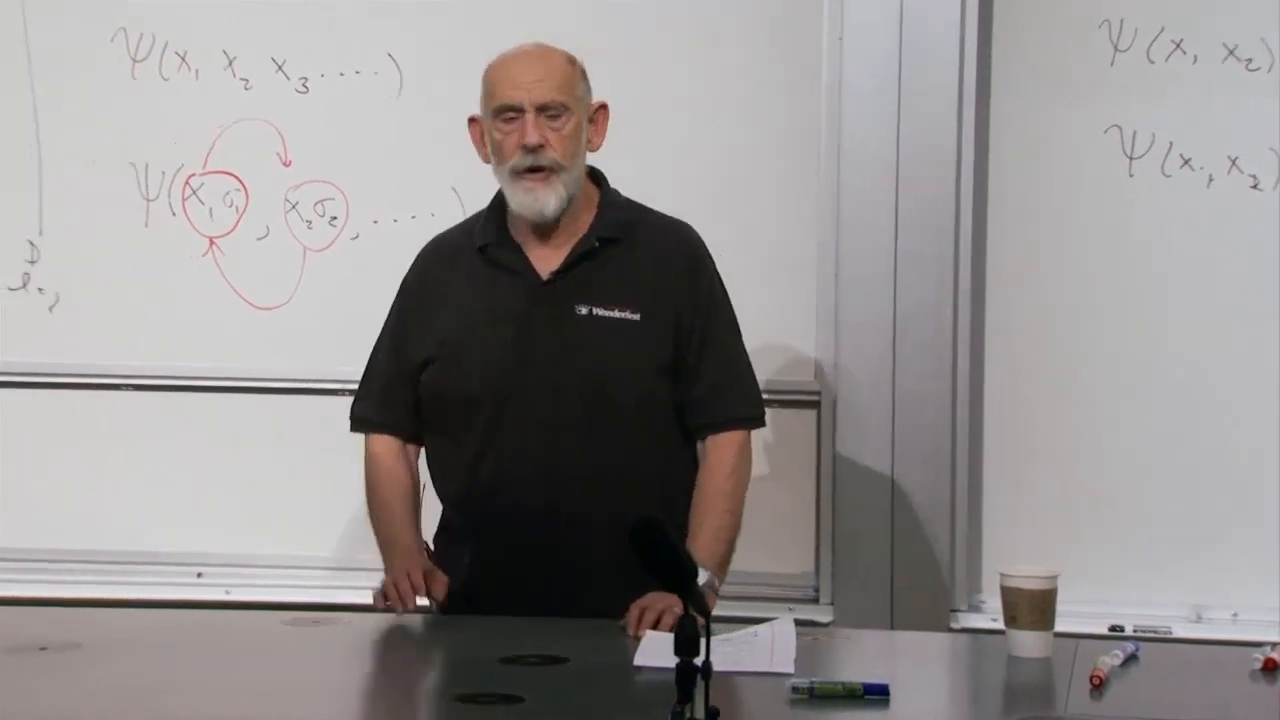
\includegraphics[width=0.9\linewidth]{lecture_05_frame_03.png}
\caption{L’échange de deux particules identiques permute leurs étiquettes complètes de position--spin. L’état bosonique reste inchangé, tandis que l’état fermionique change de signe.}
\lectureframe{00:35:25}
\end{figure}

Il s’agit de deux usages différents de la linéarité. Pour une particule,
\begin{equation}
\alpha\psi_0(x)+\beta\psi_1(x)
\end{equation}
est une superposition de deux possibilités. Pour deux particules,
\begin{equation}
\psi_0(x_1)\psi_1(x_2)
\end{equation}
est une amplitude produit dans un espace doté de deux coordonnées de particules. La symétrisation ou l’antisymétrisation combine ce produit avec son partenaire échangé.

\begin{classroomqa}
\lecturetimestamp{00:36:13}
\audiencequestion{L’échange de particules produit-il un effet d’interférence ?}
\lecturerresponse{Oui. L’annulation de l’amplitude fermionique lorsque les deux particules sont dans le même état peut se comprendre comme une interférence destructive entre les deux contributions échangées.}
\end{classroomqa}

\begin{classroomqa}
\lecturetimestamp{00:37:13}
\audiencequestion{Pauli a-t-il déduit l’exclusion à l’aide de ce même argument de symétrie ?}
\lecturerresponse{Pauli est parti d’un fait empirique et a trouvé un cadre mathématique permettant de l’exprimer. Au départ, il ne déduisait pas l’exclusion d’une théorie plus fondamentale.}
\end{classroomqa}

L’antisymétrie fournit le cadre mathématique dans lequel s’exprime la règle empirique d’exclusion.

\begin{classroomqa}
\lecturetimestamp{00:39:01}
\audiencequestion{L’interférence due à l’échange de particules est-elle liée à l’interférence entre des chemins possibles ?}
\lecturerresponse{Oui. Dans une histoire, les deux particules passent sans se croiser ; dans une autre, elles se croisent et atteignent les destinations échangées. Les amplitudes s’additionnent pour les bosons et peuvent s’annuler pour les fermions.}
\end{classroomqa}

L’échange fournit le premier signe moins. La rotation fournit le second.

\section{Le second signe moins : rotation de \texorpdfstring{\(2\pi\)}{2 pi}}

Une rotation complète semble ne rien changer. Toute direction géométrique ordinaire retrouve son orientation initiale après un angle \(2\pi\). Mais ce sont les probabilités et les valeurs moyennes qui doivent retrouver leurs valeurs initiales. Le vecteur d’état lui-même peut revenir avec une phase globale, comme cela peut aussi se produire lors d’un échange.

\begin{classroomqa}
\lecturetimestamp{00:42:12}
\audiencequestion{Quel axe utilise-t-on pour la rotation, et son générateur est-il le moment cinétique orbital, le spin, ou les deux ?}
\lecturerresponse{On peut choisir un axe extérieur ; nous prendrons ici l’axe \(z\). Le générateur est le moment cinétique total, qui comprend les contributions orbitales et de spin. Le spin lui-même n’a pas besoin d’être dirigé selon l’axe choisi.}
\end{classroomqa}

\editorialnote{Dans cette discussion, les formules du moment cinétique sont écrites avec \(\hbar=1\) ; \(m\) est donc la valeur propre sans dimension de \(J_z\).}

Soit \(\psi(\theta)\) l’état obtenu à mesure que le paramètre de rotation varie jusqu’à l’angle \(\theta\). Avec la convention utilisée ici,
\begin{equation}
J_z\psi(\theta)
=
-i\frac{\partial}{\partial\theta}\psi(\theta).
\end{equation}
Pour un état de \(J_z\) défini,
\begin{equation}
J_z\psi(\theta)=m\psi(\theta).
\end{equation}
En combinant ces équations, on obtient
\begin{equation}
-i\frac{\partial}{\partial\theta}\psi(\theta)
=
m\psi(\theta),
\end{equation}
dont la solution est
\begin{equation}
\psi(\theta)=e^{im\theta}\psi(0).
\end{equation}

Les valeurs permises de \(m\) sont des entiers ou des demi-entiers. Par conséquent,
\begin{equation}
\psi(2\pi)
=
\begin{cases}
+\psi(0), & m\in\mathbb Z,\\[4pt]
-\psi(0), & m\in\mathbb Z+\tfrac12.
\end{cases}
\end{equation}
Après un tour complet supplémentaire,
\begin{equation}
\psi(4\pi)=\psi(0)
\end{equation}
dans les deux cas. Voici le second signe moins : un état d’un multiplet de moment cinétique demi-entier change de signe lors d’une rotation de \(2\pi\).

Ce signe ne modifie pas \(\lvert\psi\rvert^2\) ; il est donc invisible lorsqu’il multiplie l’état entier. Même ainsi, une rotation de \(2\pi\) n’est pas représentée par l’identité sur un état de spin demi-entier. Cette différence devient observable lorsque le signe est relatif à une autre amplitude cohérente.

\section{Les chemins de \texorpdfstring{\(2\pi\) et \(4\pi\)}{2 pi et 4 pi}}

On peut rendre visible la différence entre \(2\pi\) et \(4\pi\) sans autre calcul. Tenez une tasse d’une main et faites-lui accomplir un tour complet sans la lâcher. La tasse retrouve son orientation initiale, mais le bras est tordu. Poursuivez d’un second tour : le bras peut alors retrouver sa position initiale sans inverser le mouvement de la tasse.

Une construction apparentée consiste à placer une sphère dans une boîte et à la relier à celle-ci par des cordes. Faire tourner la sphère de \(2\pi\) produit un enchevêtrement. Dans l’espace ordinaire à trois dimensions, l’enchevêtrement associé à un tour de \(4\pi\) peut être défait. Ce qui importe n’est pas seulement l’orientation finale de la sphère, mais le chemin parcouru dans l’espace des rotations.

\begin{classroomqa}
\lecturetimestamp{00:54:22}
\audiencequestion{Si l’on fait tourner deux fois la sphère autour du même axe, peut-on vraiment démêler les cordes ? Cela exige-t-il une dimension spatiale supplémentaire ?}
\lecturerresponse{Le chemin de \(4\pi\) peut être défait dans l’espace ordinaire à trois dimensions. Le temps paramètre le mouvement ; ce n’est pas une direction spatiale supplémentaire. Un chemin de \(2\pi\) ne peut pas être défait de cette façon, contrairement à un chemin de \(4\pi\).}
\end{classroomqa}

Les démonstrations distinguent un chemin de \(2\pi\) non trivial d’un chemin de \(4\pi\) que l’on peut défaire, sans élaborer de théorie formelle du groupe des rotations.

\section{Échange et rotation dans la représentation par une ceinture}

Les deux signes moins apparaissent maintenant côte à côte. L’échange de deux fermions identiques change le signe de leur fonction d’onde conjointe. La rotation d’un état de spin demi-entier de \(2\pi\) change elle aussi son signe. Une ceinture établit un lien géométrique entre ces deux opérations.

Disposez la ceinture de sorte que ses deux extrémités inférieures aient été échangées. Considérée autrement, la même ceinture présente une torsion de \(2\pi\). Effectuer l’échange en même temps que la rotation de \(2\pi\) supprime la torsion et laisse une ceinture sans torsion. Le processus combiné peut être ramené continûment à l’absence de toute opération.\footnote{Dans le cours, l’observation reliant l’échange--à la rotation est attribuée à David Finkelstein. La source ne précise aucune publication ; son nom est donc conservé ici uniquement comme attribution.}

\begin{classroomqa}
\lecturetimestamp{01:01:12}
\audiencequestion{S’agit-il seulement d’une affirmation sur la façon dont la ceinture est plongée dans l’espace, plutôt que d’une affirmation sur la topologie des particules ?}
\lecturerresponse{On peut interpréter la ceinture comme l’histoire d’une particule dans l’espace-temps. Si le temps s’écoule vers le haut, une coupe transversale fait apparaître des objets semblables à des particules. Des paires sont créées, un objet subit une rotation de \(2\pi\), puis deux objets identiques sont échangés. Dans cette histoire, les phases de rotation et d’échange s’annulent.}
\end{classroomqa}

Cette histoire rend explicite le calcul des phases. Partons d’une situation sans particule. En deux endroits distincts, créons une paire particule--antiparticule, ce qui laisse quatre particules à un instant intermédiaire. Faisons subir à l’une d’elles une rotation de \(2\pi\), tout en échangeant deux particules identiques ailleurs dans la configuration. L’histoire complète peut être déformée en l’histoire élémentaire où une paire est créée puis annihilée. Dans le calcul des signes considéré ici, cette histoire triviale n’ajoute aucune phase. Si \(\eta_{\mathrm{rot}}\) et \(\eta_{\mathrm{ex}}\) désignent les deux signes, l’annulation évoquée peut s’écrire simplement ainsi :\footnote{Cette équation de phase consigne l’annulation décrite entre 01:06:50 et 01:07:18 ; le cours présente cette construction comme suggestive, et non comme une preuve rigoureuse.}
\begin{equation}
\eta_{\mathrm{rot}}\eta_{\mathrm{ex}}=1.
\end{equation}

\begin{classroomqa}
\lecturetimestamp{01:03:34}
\audiencequestion{Peut-on relier l’échange aux rotations en faisant parcourir \(\pi\) à chacune de deux particules, puis en les réorientant ?}
\lecturerresponse{Cette construction peut faire intervenir des mathématiques apparentées, mais elle utilise deux rotations distinctes de \(\pi\). Le processus étudié ici comporte une seule rotation de \(2\pi\) ; les deux arguments ne sont donc pas identiques.}
\end{classroomqa}

L’argument repose sur la possibilité de créer et d’annihiler des objets semblables à des particules. Il ne prendrait pas cette forme dans une théorie où les particules seraient éternelles. Il n’est pas non plus présenté comme la preuve habituelle du théorème spin--statistiques. Son objectif est de mettre en évidence une raison topologique pour laquelle les signes associés à l’échange et à la rotation sont compatibles.

\section{Lumps, images miroir et annihilation}

On peut répéter la construction avec des configurations de champs localisées. Supposons qu’un ou plusieurs champs prennent presque partout leurs valeurs dans le vide, mais présentent une forme et une structure non nulles dans une petite région. Cette configuration localisée est un lump.

Construisons maintenant une seconde configuration, image miroir appropriée de la première. Appelons l’une la particule et l’autre l’antiparticule. Rapprochons-les. Les parties correspondantes des configurations de champs se rencontrent et s’annulent mutuellement. À une étape intermédiaire, certaines parties des lumps peuvent déjà avoir disparu tandis que d’autres subsistent. En poursuivant la déformation, on élimine la structure restante et l’on ramène les champs à la configuration du vide. Deux torsions orientées en sens opposés dans une ceinture donnent la même image : rapprochez-les par poussée et elles se défont.

On peut inverser le processus. L’espace vide peut produire un lump et son partenaire miroir. On peut créer deux paires de ce type, faire subir à un lump une rotation de \(2\pi\), échanger deux lumps identiques, puis annihiler de nouveau les paires. La même annulation entre échange--et rotation s’applique alors. Cette extension de la construction reste heuristique ; ce n’est pas un théorème concernant toute excitation localisée.

\begin{classroomqa}
\lecturetimestamp{01:11:30}
\audiencequestion{Existe-t-il des réalisations physiques de ces configurations de champs semblables à des lumps ?}
\lecturerresponse{Oui. On peut citer les noyaux dans les descriptions de type Skyrmion, les monopôles magnétiques et d’autres excitations des champs semblables à des particules.}
\end{classroomqa}

L’image des lumps miroirs rend la généralisation intelligible. Ce qui compte, ce n’est pas que l’objet ait été initialement une particule ponctuelle élémentaire, mais qu’une excitation semblable à une particule et son partenaire puissent être créés, rapprochés et annihilés de façon continue. Cette propriété motive une relation plus générale entre le comportement sous rotation et sous échange.

\begin{classroomqa}
\lecturetimestamp{01:16:12}
\audiencequestion{Le spin un demi signifie-t-il que l’état n’accumule que la moitié de la phase de rotation habituelle ?}
\lecturerresponse{Dans cette convention, la phase est \(e^{im\theta}\). Pour un \(m\) demi-entier, une rotation de \(2\pi\) donne \(-1\), tandis qu’une rotation de \(4\pi\) donne \(+1\).}
\end{classroomqa}

\section{Un signe global et une expérience nulle}

Peut-on observer le signe moins issu d’une rotation de \(2\pi\) ? Commençons par une expérience où ce n’est pas possible. Piégeons un électron dans un champ magnétique, laissons son spin suivre le champ tandis que l’appareil tourne lentement de \(2\pi\), puis libérons l’électron dans un dispositif d’interférence. Comparons cela à la même procédure sans rotation.

La rotation transforme l’état selon
\begin{equation}
\psi\longmapsto-\psi,
\end{equation}
mais le signe moins multiplie l’état entier. Toutes les probabilités restent inchangées ; la figure d’interférence finale ne conserve donc aucune trace de la rotation préalable. C’est une expérience nulle : une phase commune n’a rien avec quoi interférer.

\begin{classroomqa}
\lecturetimestamp{01:20:01}
\audiencequestion{Pourquoi faut-il faire tourner lentement le champ magnétique ?}
\lecturerresponse{Le spin doit continuer à suivre le champ magnétique en rotation. Si le champ est entraîné trop rapidement, le spin ne restera pas aligné sur lui.}
\end{classroomqa}

\section{Un électron dans deux branches cohérentes}

Le signe devient observable lorsqu’il est rendu relatif. Faisons passer un électron dans un séparateur de faisceau. Une partie de sa fonction d’onde suit un trajet, l’autre partie un second trajet :
\begin{equation}
\psi(x)=\psi_1(x)+\psi_2(x).
\end{equation}
Il s’agit d’un seul électron, pas de deux électrons. C’est une superposition cohérente de deux possibilités. Il faut bien garder cette distinction à l’esprit : les deux paquets ne sont pas deux particules indépendantes.

Dirigeons les deux paquets vers des régions distinctes contenant des champs magnétiques. Dans l’une, faisons tourner le champ de \(2\pi\), sans modifier l’autre. Pour un état de spin demi-entier,
\begin{equation}
\psi_1(x)+\psi_2(x)
\longmapsto
\psi_1(x)-\psi_2(x),
\end{equation}
où l’on a choisi \(2\) comme étiquette de la branche ayant subi la rotation. Le signe est maintenant relatif. Lorsque les deux paquets se recouvrent plus tard, l’addition devient une soustraction. Un point d’interférence constructive peut devenir un point d’interférence destructive, voire un nœud.

\begin{classroomqa}
\lecturetimestamp{01:23:46}
\audiencequestion{Que fait-on tourner s’il n’y a qu’un électron mais deux branches de la fonction d’onde ?}
\lecturerresponse{L’électron est dans une superposition cohérente de deux possibilités localisées. On fait subir une rotation à une branche, pas à l’autre. Si l’on ouvre les boîtes pour savoir laquelle des deux possibilités s’est réalisée, cette mesure détruit l’interférence.}
\end{classroomqa}

Ouvrir les boîtes ne révélerait qu’un seul électron, dans l’une ou l’autre. Sans cette mesure, les deux amplitudes restent présentes dans l’état. La répétition de l’expérience fait apparaître la figure d’interférence détection après détection. Au nœud produit par le signe moins relatif, aucun électron n’est détecté.

\section{Précession magnétique et interférence à deux fentes}

Un dispositif schématique plus pratique remplace l’expérience des boîtes, qui exigerait un mouvement très lent. Séparons une onde électronique cohérente en deux trajets. Sur l’un d’eux, faisons passer l’électron dans une région magnétique alors que son spin est initialement transverse au champ. Le spin entre alors en précession. En choisissant l’intensité du champ et le temps de traversée, on peut faire accomplir au spin de cette branche un tour complet de \(2\pi\), tandis que l’autre branche n’effectue aucun tour de ce type.\footnote{Le cours indique qu’une expérience apparentée sur la phase des spineurs a été réalisée et en décrit le principe, mais la source ne précise ni publication ni dispositif particulier. Le compte rendu se limite donc à la construction présentée dans le cours.}

\begin{classroomqa}
\lecturetimestamp{01:27:05}
\audiencequestion{Comment peut-on déterminer le trajet suivi par l’électron unique ?}
\lecturerresponse{On ne le peut pas sans compromettre l’expérience. Toute mesure qui enregistre le trajet suivi par l’électron détruit l’interférence.}
\end{classroomqa}

\begin{classroomqa}
\lecturetimestamp{01:27:50}
\audiencequestion{Qu’est-ce exactement qu’une branche de la fonction d’onde, et comment le séparateur en produit-il deux ?}
\lecturerresponse{Une branche est un paquet d’ondes localisé le long d’un trajet. Le séparateur transforme l’onde incidente en deux paquets spatialement séparés, que des champs électriques ou magnétiques peuvent guider sur des trajets différents.}
\end{classroomqa}

À part la région magnétique, il s’agit de l’expérience à deux fentes. Une onde électronique incidente se sépare en deux paquets. Les ondes sortantes s’étalent dans une région de détection commune, où leurs amplitudes se recouvrent. En l’absence de rotation relative, les amplitudes centrales peuvent s’additionner. Une rotation de spin de \(2\pi\) sur l’un des trajets inverse une amplitude et peut annuler ces mêmes contributions.

\begin{classroomqa}
\lecturetimestamp{01:30:46}
\audiencequestion{Comment peut-il y avoir interférence si l’électron emprunte des tubes ou des fentes distincts ?}
\lecturerresponse{La détection finale ne révèle pas le trajet. Les deux amplitudes d’onde sortantes s’étalent et se recouvrent au détecteur. Chercher à déterminer le trajet suivi détruirait l’interférence.}
\end{classroomqa}

\begin{classroomqa}
\lecturetimestamp{01:33:22}
\audiencequestion{Le diamètre du tube ou de la fente doit-il être comparable à la longueur d’onde de l’électron ?}
\lecturerresponse{Dans une réalisation littérale de l’expérience à deux fentes fondée sur la diffraction, l’ouverture doit être assez petite pour produire l’étalement nécessaire. Le dispositif décrit est schématique et ne constitue pas un plan expérimental pratique.}
\end{classroomqa}

\begin{classroomqa}
\lecturetimestamp{01:33:44}
\audiencequestion{Une rotation de polarisation correspondante des photons de \(2\pi\) laisserait-elle la figure d’interférence inchangée ?}
\lecturerresponse{Oui. Les photons ont un spin entier ; une rotation complète de \(2\pi\) n’introduit donc pas le signe moins propre aux fermions.}
\end{classroomqa}

\begin{classroomqa}
\lecturetimestamp{01:34:12}
\audiencequestion{En quoi l’expérience pratique s’écarte-t-elle légèrement de la version idéalisée ?}
\lecturerresponse{Dans le dispositif idéal, le spin tourne de manière adiabatique. Dans la description pratique, l’électron traverse une région magnétique et son spin précesse plus rapidement, mais la phase mesurée reste celle qui est associée à un tour de \(2\pi\).}
\end{classroomqa}

Le dispositif lent isole l’idée en veillant à ce que le spin suive le champ sans mouvement supplémentaire. Le dispositif fondé sur la précession produit dynamiquement le même signe relatif. Dans les deux versions, les deux trajets doivent cesser d’être distinguables pour qu’une figure d’interférence puisse apparaître.

\begin{classroomqa}
\lecturetimestamp{01:36:15}
\audiencequestion{Faut-il recombiner les deux branches après le séparateur ?}
\lecturerresponse{Oui. Les paquets d’ondes qui émergent doivent se recouvrir, ou s’étendre sur une même région de détection, afin que leurs amplitudes puissent former une figure d’interférence.}
\end{classroomqa}

\begin{classroomqa}
\lecturetimestamp{01:38:12}
\audiencequestion{Cette expérience de rotation avec un seul électron découle-t-elle du principe d’exclusion de Pauli ?}
\lecturerresponse{Non. Il n’y a qu’un seul électron. L’expérience mesure la phase du spineur lors d’une rotation, et non l’exclusion de deux fermions d’un même état.}
\end{classroomqa}

\section{Interférence par échange et rotation relative}

On pourrait mettre en évidence un signe d’échange par la même méthode générale, bien que l’appareillage proposé soit plus complexe. On commence par deux électrons et l’on sépare leur fonction d’onde commune en deux branches cohérentes. Il n’y a toujours que deux électrons, et non quatre : la paire suit l’une ou l’autre des deux possibilités. Dans une branche, on échange les deux électrons ; dans l’autre, on ne les échange pas. Une fois les branches recombinées, le signe d’échange fermionique apparaît comme une phase relative et peut modifier les interférences.

La proposition finale compare directement les deux signes moins. Une branche acquiert la phase d’échange fermionique, tandis que l’autre acquiert la phase correspondante à une rotation de \(2\pi\). Les deux phases valent \(-1\), si bien que leurs effets relatifs s’annulent.\footnote{L’enregistrement entre 01:40:26 et 01:41:15 montre clairement une phase d’échange, une phase correspondant à une rotation de \(2\pi\) et leur annulation, mais les paroles disponibles ne permettent pas de déterminer à quoi la rotation est précisément attribuée.} Le cours présente cela comme une expérience de pensée proposée et précise qu’à la connaissance de l’intervenant, elle n’avait pas été réalisée.

\begin{classroomqa}
\lecturetimestamp{01:41:34}
\audiencequestion{L’observation d’une phase d’échange remettrait-elle en question l’indiscernabilité des deux électrons ?}
\lecturerresponse{Non. L’indiscernabilité quantique est plus subtile que la similitude classique. Elle permet au vecteur d’état de changer de signe lors d’un échange, même si aucune étiquette observable ne distingue les particules.}
\end{classroomqa}

Il reste une dernière réserve. Faire tourner un monde entier isolé de \(2\pi\) ne produirait qu’une phase commune, qu’aucune expérience interne ne pourrait révéler. L’expérience détectable consiste à faire tourner une branche cohérente par rapport à une autre. Ce qui est observé n’est donc pas un signe absolu, mais les interférences produites par un signe relatif.
